\documentclass[12pt, a4]{report}
    \usepackage[utf8]{inputenc}
    \usepackage[croatian]{babel}
    \usepackage{graphicx}
    \usepackage[a4paper, total={6in, 10in}]{geometry}
    \usepackage{caption}
    \usepackage{amsmath}
    \usepackage{subfig}

    \graphicspath{ {res/} }

    \title{Laboratorijska vježba 3}
    \author{Matija Marić, 0036479678}
    \date{\today}

\begin{document}
\begin{titlepage}
	\maketitle
\end{titlepage}

\tableofcontents{}

\chapter{Obnavljanje slike}
\section{Modeliranje degradiranja slike kao FIR filtera}
\begin{enumerate}
	\item
	      \begin{minipage}{\linewidth}
		      \centering
		      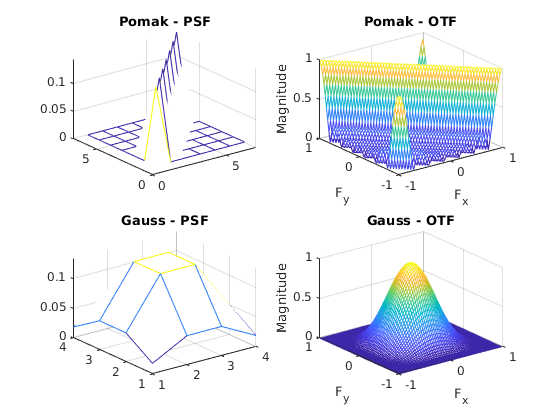
\includegraphics[width=0.75\textwidth]{zad01}
		      \captionof{figure}{PSF i OTF karakterističnih zamućenja}
	      \end{minipage}
	\item
	      \begin{minipage}{\linewidth}
		      \centering
		      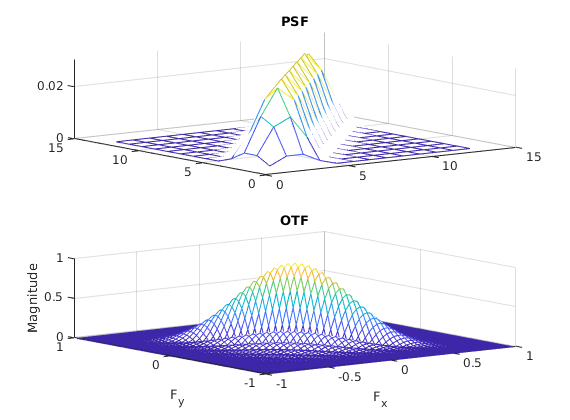
\includegraphics[width=0.75\textwidth]{zamcomb}
		      \captionof{figure}{PSF i OTF kombinacije zamućenja}
	      \end{minipage}
	\item
	      \begin{minipage}{\linewidth}
		      \centering
		      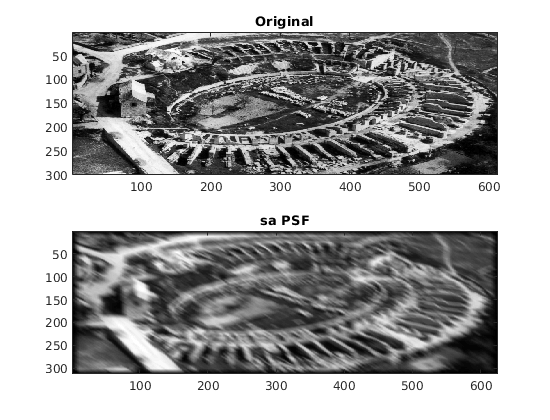
\includegraphics[width=0.75\textwidth]{salonapsf}
		      \captionof{figure}{PSF na slici {\it salona.png}}
	      \end{minipage}
	\item
	      \begin{minipage}{\linewidth}
		      \centering
		      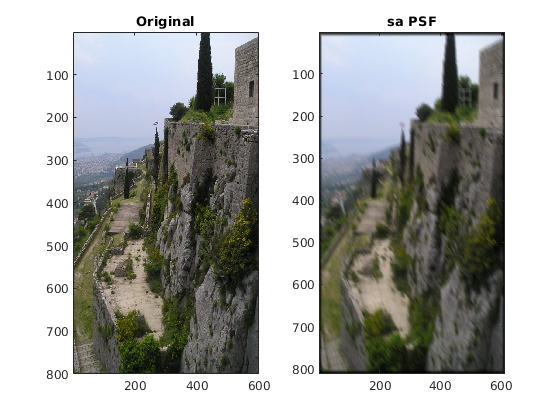
\includegraphics[width=0.75\textwidth]{klispsf}
		      \captionof{figure}{PSF na slici {\it klis.png}}
	      \end{minipage}
\end{enumerate}

\section{Inverzni filter}
\begin{enumerate}
	\item
	      \begin{minipage}{\linewidth}
		      \centering
		      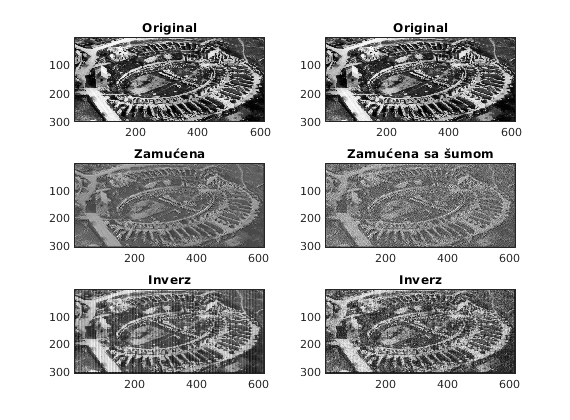
\includegraphics[width=0.75\textwidth]{inverse}
		      \captionof{figure}{Inverzno filtrirana slika sa i bez aditivnog šuma.}
	      \end{minipage}
	\item
	      Srednja kvadratna greška bez šuma je 0.0057, a sa šumom 0.0121.

	\item
	      \begin{minipage}{\linewidth}
		      \centering
		      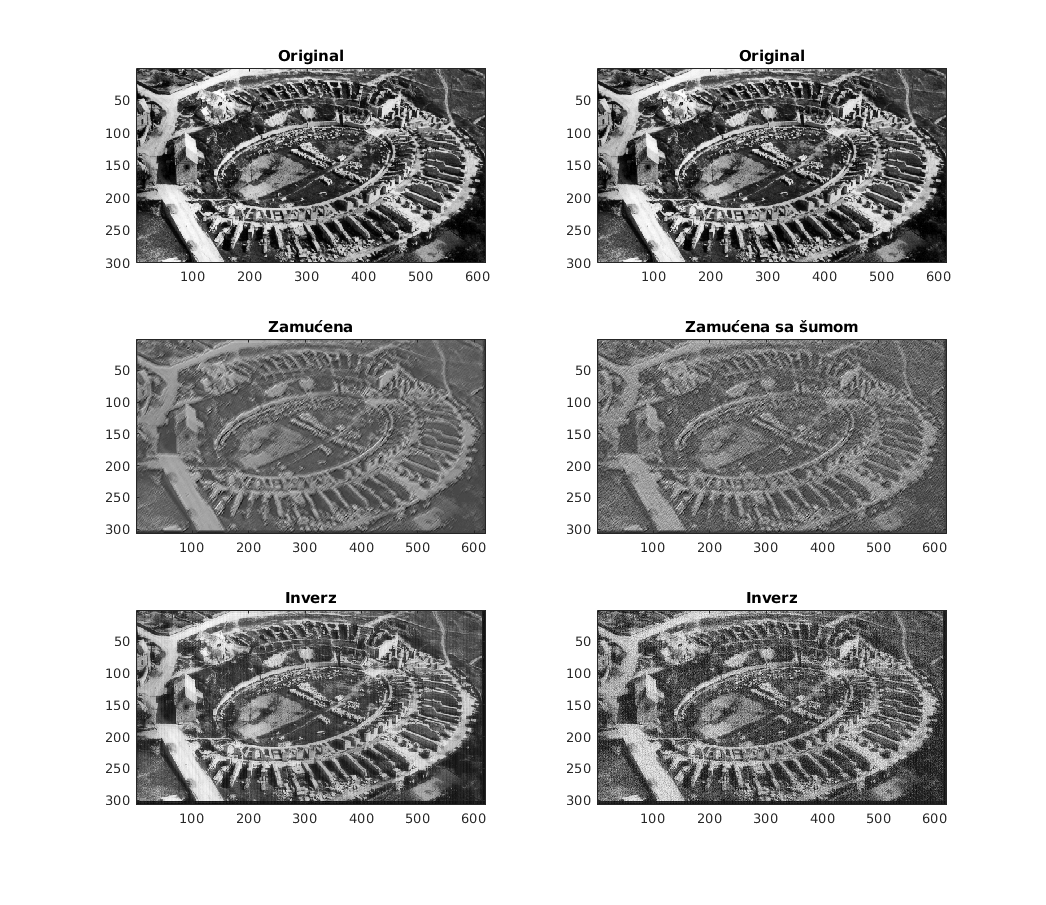
\includegraphics[width=0.75\textwidth]{inversequant}
		      \captionof{figure}{Inverzno filtrirana slika sa i bez aditivnog šuma i kvantizirano na 256 razina.}
	      \end{minipage}
	\item
	      Srednja kvadratna greška sa kvantizacijom bez šuma je 0.0016, a sa šumom 0.0121. Kvantizacijom se smanjuje greška.
\end{enumerate}

\section{Pseudoinverzni filter}
\begin{enumerate}
	\item
	      \begin{minipage}{\linewidth}
		      \centering
		      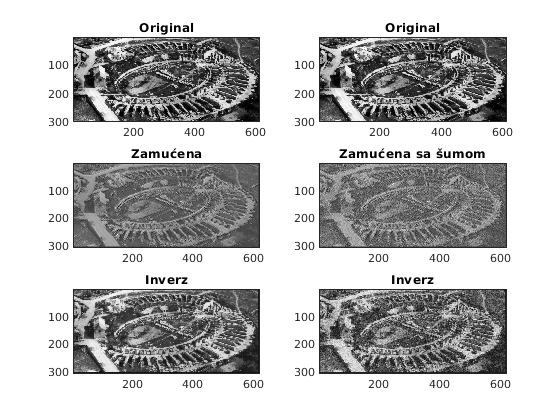
\includegraphics[width=0.75\textwidth]{pseudoinverse}
		      \captionof{figure}{Pseudoinverzno filtrirana slika sa i bez aditivnog šuma, sa $K = 0.05$.}
	      \end{minipage}
	\item
	      Srednja kvadratna greška bez šuma je 0.0013, a sa šumom 0.0112.
	\item
	      Pseudoinverzno filtriranje daje bolje rezultate.
	\item
	      \begin{minipage}{\linewidth}
		      \centering
		      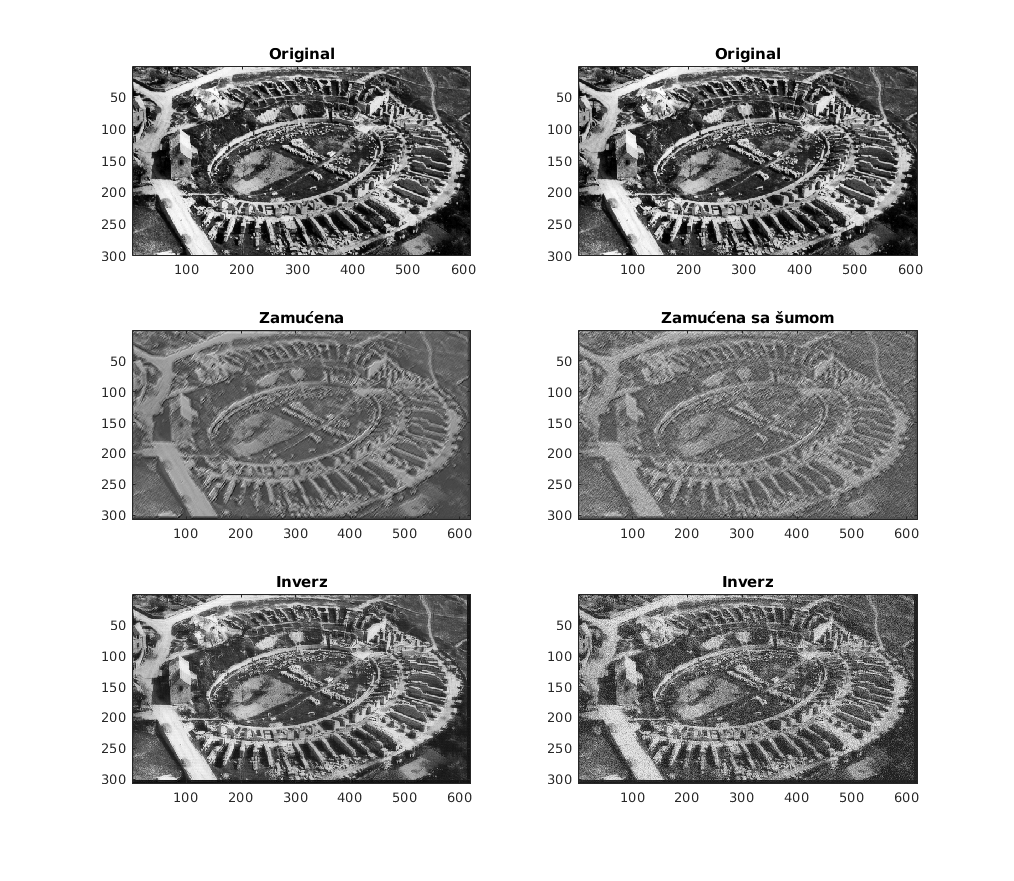
\includegraphics[width=0.75\textwidth]{pseudoinversequant}
		      \captionof{figure}{Pseudoinverzno filtrirana slika sa i bez aditivnog šuma, sa $K = 0.05$ i kvantizirano na 256 razina.}
	      \end{minipage}
	\item
	      Srednja kvadratna greška bez šuma je 0.0013, a sa šumom 0.0112.
	\item
	      Pseudoinverzno filtriranje daje bolje rezultate.
	\item
	      Kvantizacija kod pseudoinverznog filtriranje ne radi nikakvu razliku u rezultatima.
\end{enumerate}

\section{Wienerov filter}
\begin{enumerate}
	\item
	      \begin{minipage}{\linewidth}
		      \centering
		      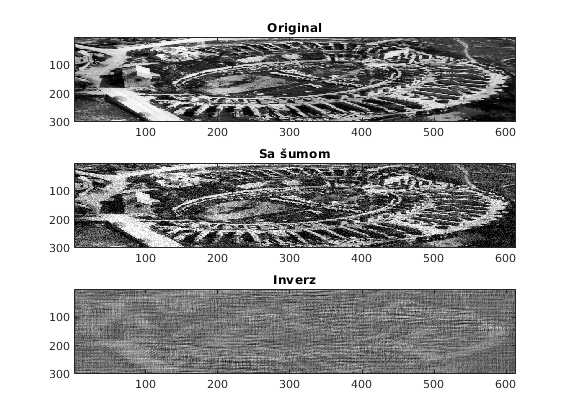
\includegraphics[width=0.75\textwidth]{weinernoise}
		      \captionof{figure}{Slika sa aditivnim šumom filtrirana Weinerovim filterom.}
	      \end{minipage}
	\item
	      \begin{minipage}{\linewidth}
		      \centering
		      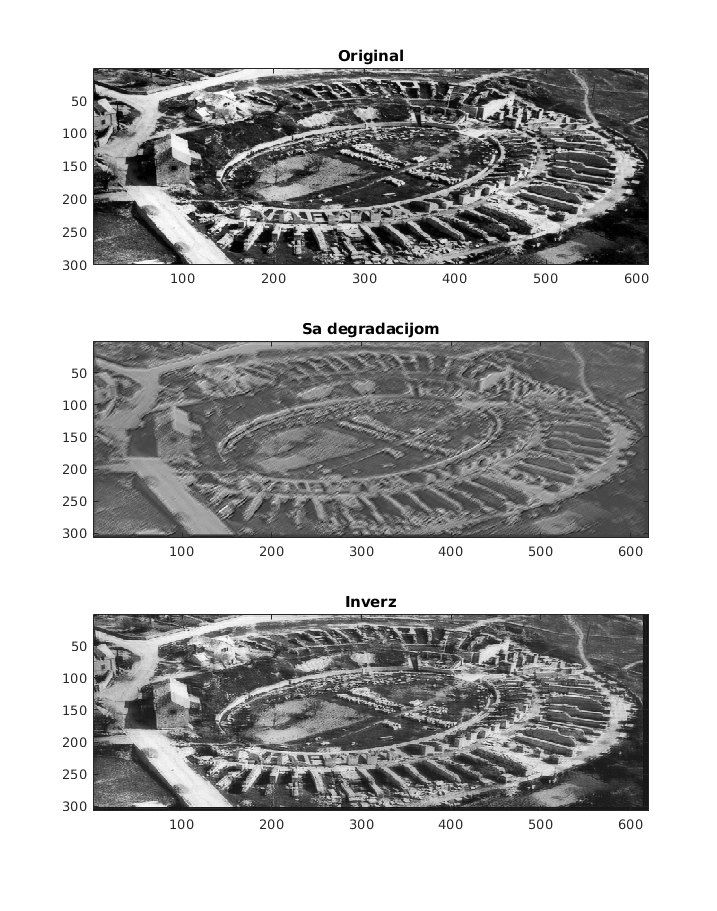
\includegraphics[width=0.75\textwidth]{weinerpsf}
		      \captionof{figure}{Slika sa degradacijom bez šuma filtrirana Weinerovim filterom.}
	      \end{minipage}
	\item
	      \begin{minipage}{\linewidth}
		      \centering
		      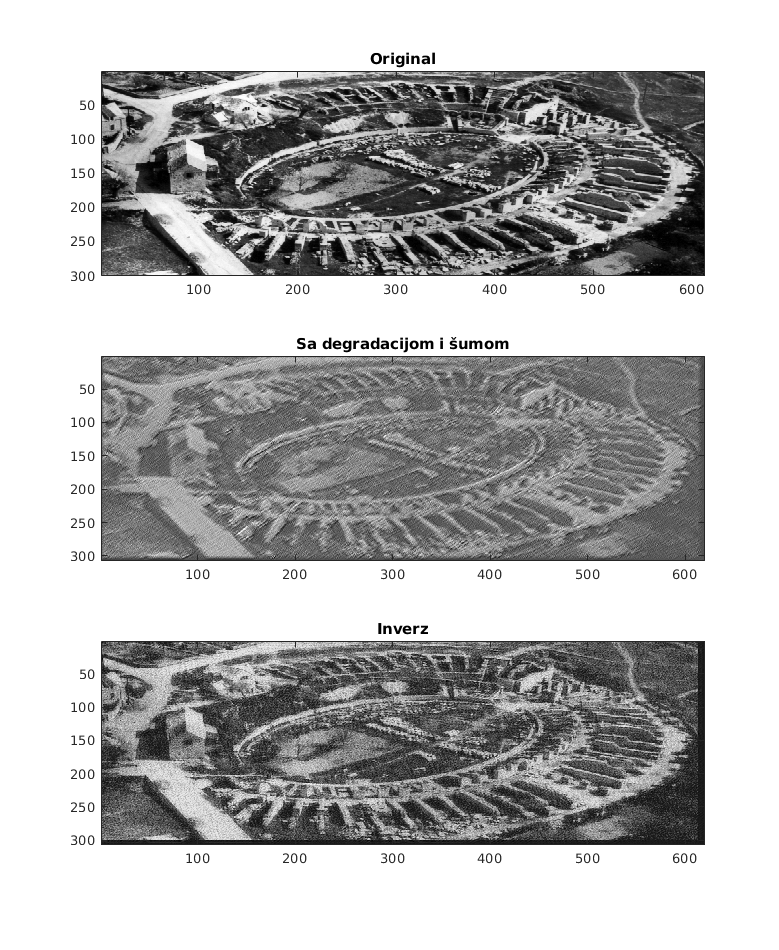
\includegraphics[width=0.75\textwidth]{weinernpsf}
		      \captionof{figure}{Slika sa degradacijom i šumom filtrirana Weinerovim filterom.}
	      \end{minipage}
	\item
	      Srednja kvadratna greška za sliku sa šumom je 0.1307, sa degradacijom 0.0017, sa degradacijom i šumom 0.0106.
	\item
	      Weinerov filter daje bolje rezultate od inverznog i pseudoinverznog filtera.
	\item
	      Odnos signal/šum za sliku sa šumom je 1.2552, sa degradacijom 1.0819, sa degradacijom i šumom 1.0477.
\end{enumerate}

\subsection{Autokorelacijska funkcija}
\begin{enumerate}
	\item
	      \begin{minipage}{\linewidth}
		      \centering
		      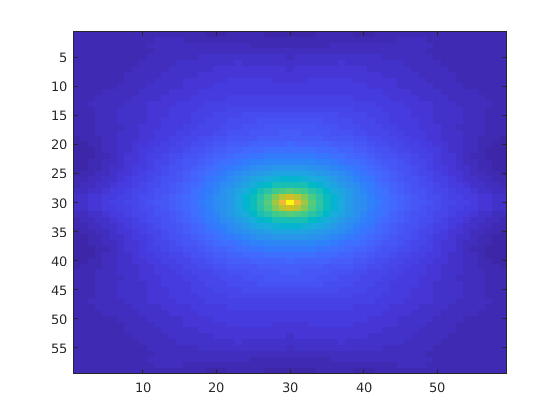
\includegraphics[width=0.75\textwidth]{akfgauss}
		      \captionof{figure}{Autokorelacijska funkcija slike degradirane Gaussovim šumom.}
	      \end{minipage}


\end{enumerate}

\chapter{Pronalaženje značajki slike}
\section{Amplitudne značajke slike}
\begin{enumerate}
	\item
	      \begin{minipage}{\linewidth}
		      \centering
		      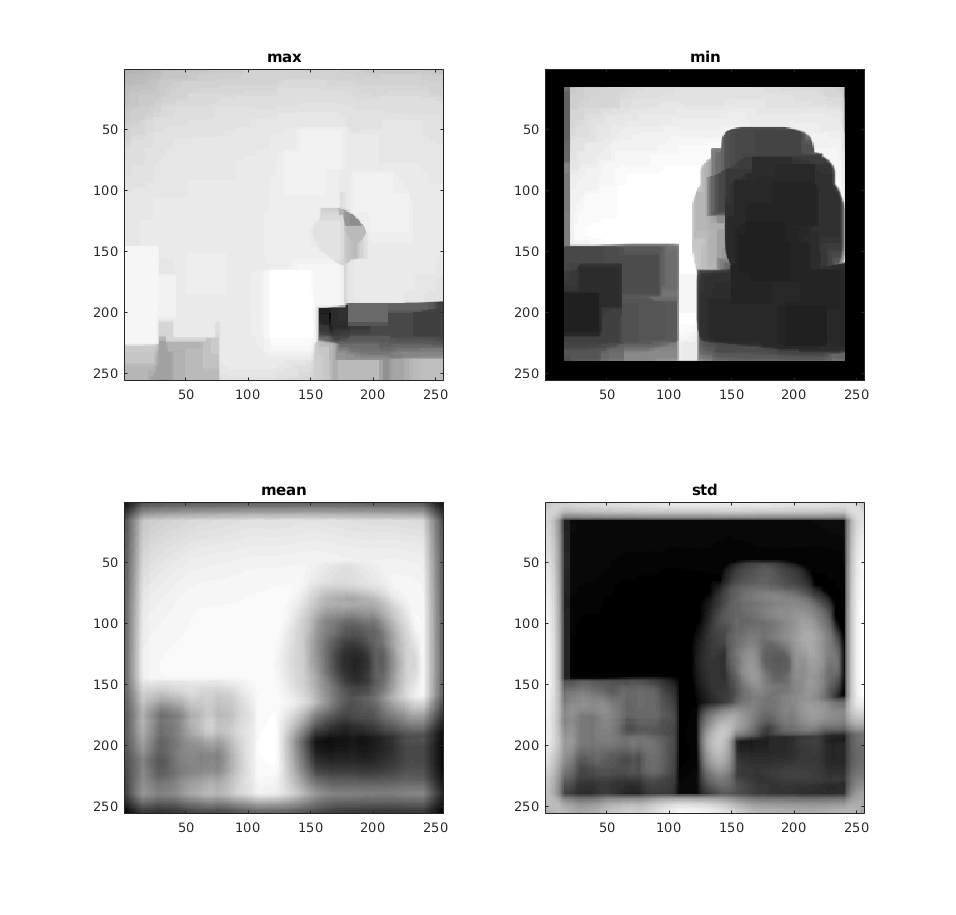
\includegraphics[width=0.75\textwidth]{ampfeat}
		      \captionof{figure}{Amplitudne značajke slike {\it clock.tiff}, blok veličine $32\times32$}
	      \end{minipage}
	      \begin{minipage}{\linewidth}
		      \centering
		      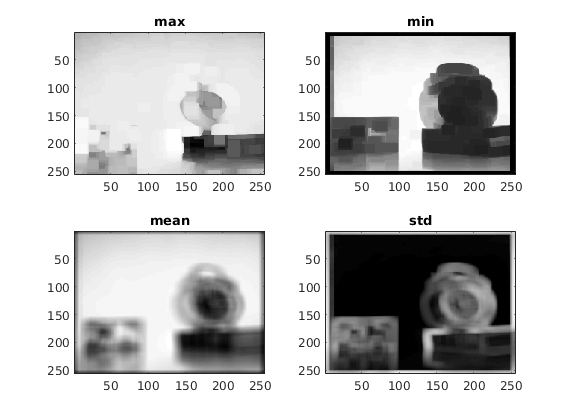
\includegraphics[width=0.75\textwidth]{ampfeat16}
		      \captionof{figure}{Amplitudne značajke slike {\it clock.tiff}, blok veličine $16\times16$}
	      \end{minipage}
	      \begin{minipage}{\linewidth}
		      \centering
		      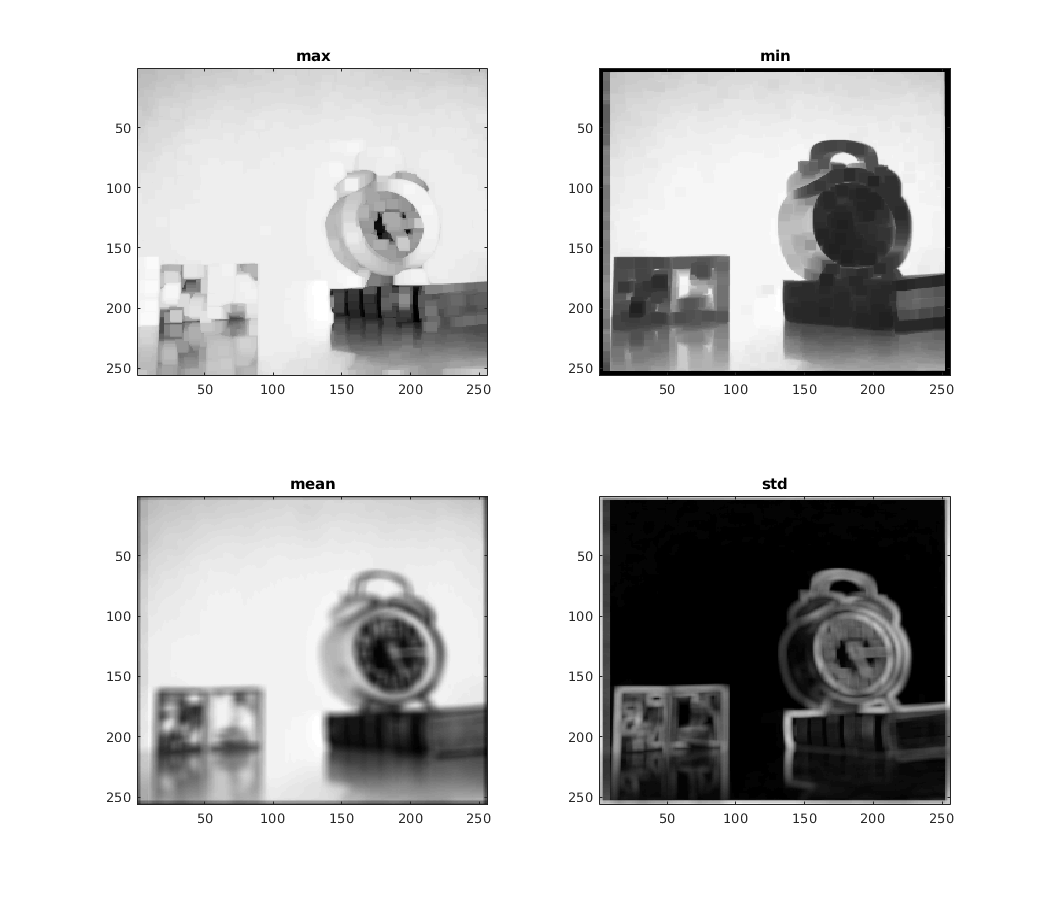
\includegraphics[width=0.75\textwidth]{ampfeat8}
		      \captionof{figure}{Amplitudne značajke slike {\it clock.tiff}, blok veličine $8\times8$}
	      \end{minipage}

\end{enumerate}

\section{Značajke histograma prvog reda}
\begin{enumerate}
    \item 
        \begin{minipage}{\linewidth}
            \centering
            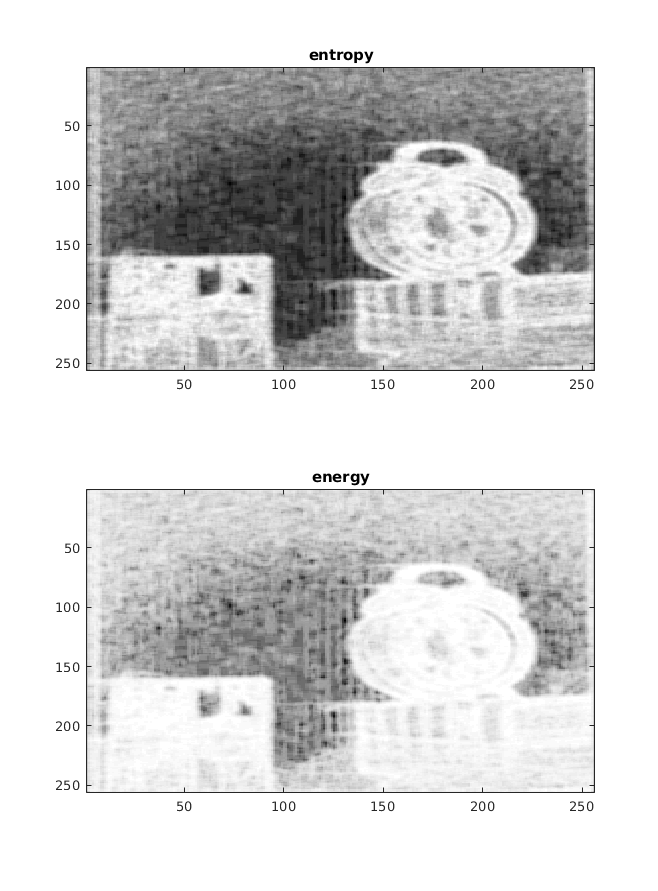
\includegraphics[width=0.75\textwidth]{hist1}
            \captionof{figure}{Značajke histograma prvog reda (entropija i energija) slike {\it clock.tiff}, blok veličine $5\times5$}
        \end{minipage}
    
\end{enumerate}

\section{Značajke histograma drugog reda}
\begin{enumerate}
    \item
        \begin{minipage}{\linewidth}
            \centering
            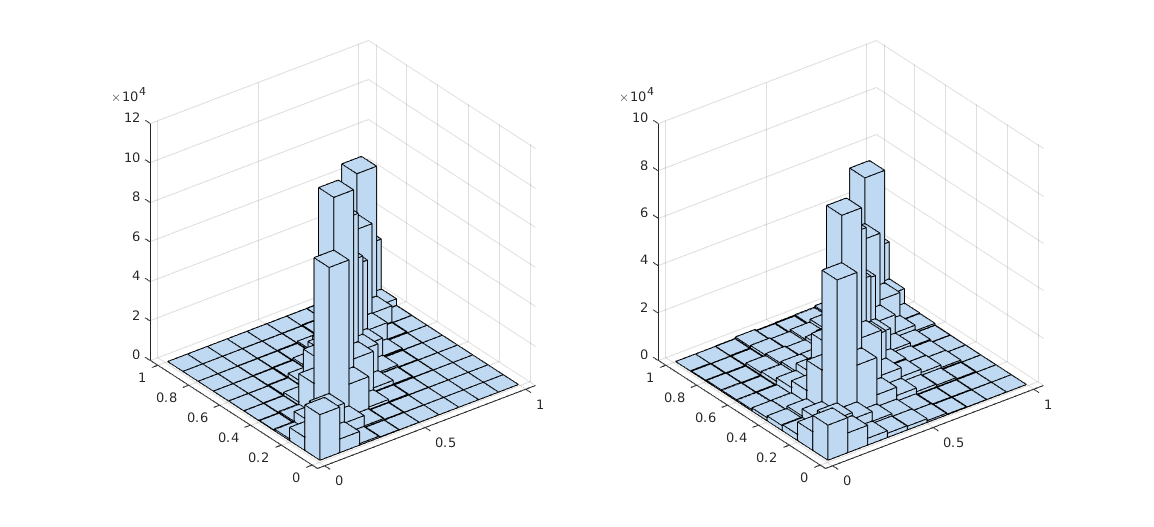
\includegraphics[width=0.75\textwidth]{hist2}
            \captionof{figure}{Histogrami drugog reda za pomake (1, 1) i (5, 5)}
        \end{minipage}
    \item
        Rezultati su grupirani oko dijagonale jer su slike pomaknute jednako na svakoj osi.
    \item
        Kod drugog histograma rezultati su raspršeniji jer je veći pomak i jača korelacija za raspršenije piksele.
    \item
        Veliki dio piksela na slici {\it saturn.tif} su crni i pomakom većina ostaje ista, zato je najveći stupac na (0, 0) poziciji u histogramu.


        \begin{minipage}{\linewidth}
            \centering
            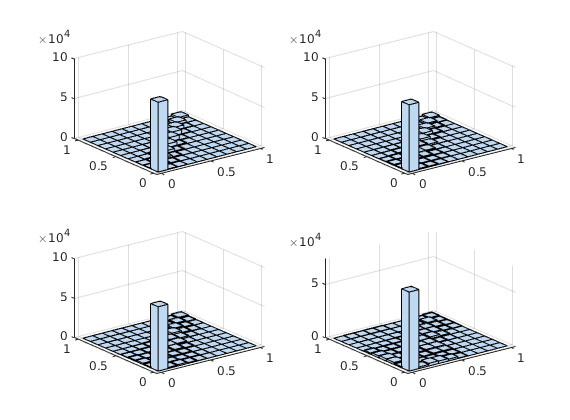
\includegraphics[width=0.75\textwidth]{saturnhist}
            \captionof{figure}{Histogrami drugog reda za pomake (1, 1), (3, 3), (5, 5), (10, 10) slike {\it saturn.tif}}
        \end{minipage}

\section{Sobelov i Prewittov operator}
\begin{enumerate}
    \item
        \begin{minipage}{\linewidth}
            \centering
            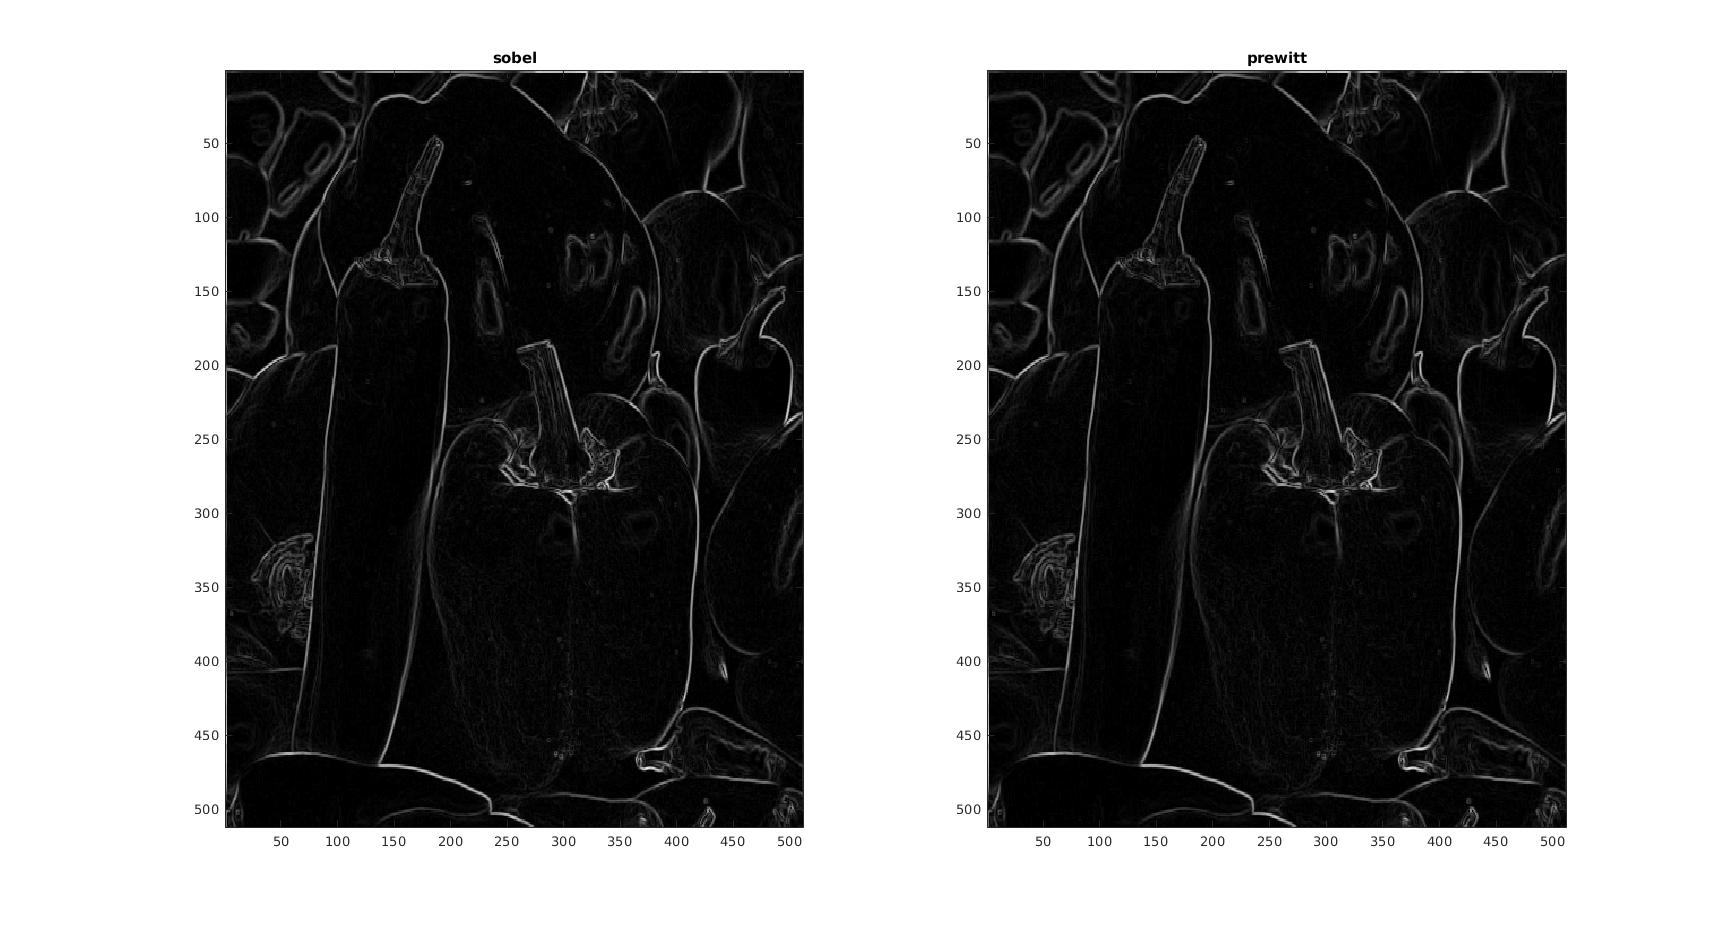
\includegraphics[width=0.75\textwidth]{edge}
            \captionof{figure}{Procjene gradijenta Sobelovim i Prewittovim operatorom na slici {\it 4.2.07.tiff}}
        \end{minipage}
    

    
\end{enumerate}
\end{enumerate}


\end{document}